\chapter{Senzory a akční plány}

\section{Motivace}
V této kapitole se již přesouváme od hry samotné ke způsobu, jak na daný stav hry nahlížet strojově a také, jak na stav strojově reagovat. 
Na nejnižší úrovni dostávají agenti od prostředí stav, který obsahuje seznamy všech vesmírných objektů a agenti na to mají reagovat nějakou elementární akcí.
Bylo by proto dobré vymyslet princip, jak z obsáhlých a detailních informací nízké úrovně získávat menší objemy potřebnějších informací vyšší úrovně. 
A podobně by se nám mohlo hodit místo elementárních akcí nízké úrovně, vymyslet princip jak volit akce tak, aby vedly k akcím vyšší úrovně.
A právě tyto abstrakce realizujeme pomocí senzorů a akčních plánů.
\subsection{Senzor}

Senzorem nazveme metodu, která nám z kompletního stavu reprezentovaného seznamem vesmírných objektů extrahuje nějakou užitečnou informaci, která není ve stavu explicitně zadána.
Informace získané z těchto senzorů, respektive senzorických metod, můžeme využít v rozhodovacím problému vybrání akcí.
Většina senzorických metod využívá simulování hry. Na základě současného rozpoložení vesmírných objektů se v rámci simulace pokračuje v jejich pohybu, tak jak by se pohybovaly, pokud by žádný z hráčů neprováděl žádné akce.
A na základě toho, co se v simulaci stane v nejbližších krocích hry, můžeme zjistit konkrétní informace, které platí o současném stavu hry.
V simulaci žádný z hráčů neprovádí žádné akce, kromě těch, na jejichž dopad se v dané simulaci dotazujeme.
Všechny simulace probíhají omezený počet kroků. Tento počet kroků je roven konstantě \emph{\uppercase{Impact\_radius}}. Pro tuto hodnotu se mi ukázal být vhodný počet 25.
Je to dostatečně vysoká hodnota, aby senzory včas zaznamenaly potřebné informace a zároveň je dostatečně nízká, aby senzory nebyly zbytečně výpočetně náročné.


\subsubsection{Příklady senzorů}
\begin{itemize}
    \item \bf{První sražený neutrální asteroid} - Zde se simuluje pohyb vesmírné lodi, střel a neutrálních asteroidů. 
    V případě, že v simulaci dojde k srážce vesmírné lodi a neutrálního asteroidu, vrací tento senzor daný asteroid a počet kroků, po kterém došlo ke srážce.
    Berou se zde v úvahu i vlastní střely. Pokud dojde k sestřelení asteroidu střelou, jsou jak asteroid, tak i střela odstraněny ze simulace.
    \item První sražený nepřátelský asteroid - Jde o téměř identický senzor, jen s rozdílem, že se nesoustředí na asteroidy neutrální, ale na asteroidy nepřátelské.
    \item Asteroid zasáhne nepřátelskou loď - Zde se simuluje pouze pohyb konkrétního asteroidu a nepřátelské lodí. 
    Opět je zde nastaven daný limit na počet simulovaných kroků. 
    Senzor vrací informaci zda, a v kolika krocích se střetl s nepřátelskou lodí.
    V simulaci nepřátelská loď neprovádí žádné reakce.
    \item Střela zasáhne konkrétní asteroid - Jde o simulaci podobnou předchozí. Simuluje se pohyb konkrétního asteroidu a konkrétní střely.
    \item Střela zasáhne libovolný asteroid - Simuluje se pohyb konkrétní střely a všech neutrálních a nepřátelských asteroidů.
        Tato senzorická metoda vrací zda střela zasáhla sestřelila asteroid, daný asteroid a počet kroků, po kterém střela sestřelila asteroid.
    \item Vzdálenost dvou bodů - Vrátí vzdálenost vyjádřenou v Euklidovské metrice.
    \item Přepočítání nejbližší polohy asteroidu od vesmírné lodi - Vzhledem k tomu, že prostor je jistým způsobem cyklický, tak v případě, že nás zajímá nejkratší vzdálenost asteroidu od vesmírné lodi, tak přímá vzdálenost těchto objektů, tak jak jsou graciky objekty zobrazeny v herním prostoru, nemusí být nejkratší.
        Musíme vzít v úvahu všechny čtyři polohy asteroidu, které získáme postupným posunutím asteroidu o šířku a délku prostoru.
        Jinak řečeno, vzdálenost souřadnice asteroidu posunutého přes hranici prostoru může být kratší než přímá vzdálenot k původní souřadnici asteroidu.
    \item N nejblizších asteroidů od vesmírné lodi - Tento senzor spočítá nejkratší vzdálenosti vesmírné lodi ke všem asteroidům ve hře a vrátí relativní polohu N nejbližších z nich k vesmírné lodi.
    
\end{itemize}


\begin{figure}[p]

    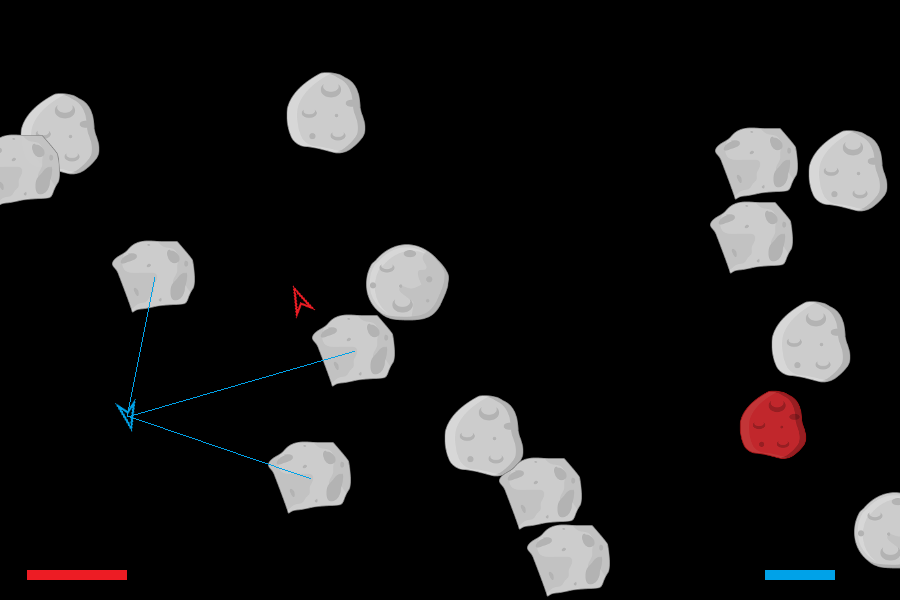
\includegraphics[width=150mm, height=100mm]{./Obrazky/N_nearest_asteroids.png}
    \caption{Ukázka senzoru "N nejbližších asteroidů od vesmírné lodi" pro N=3}
    \label{obr02:}
    \end{figure}


\subsection{Akční plán}


\section{Jednotliv plány}
\subsection{Útok}
\subsection{Sestřelující obrana}
\subsection{Úhybná obrana}
\subsection{Zastavení letu}




